\documentclass%
%[handout]
{beamer}
% % % % % % % %
% % % % % % % %
% % % % % % % %
%IMPORTANT
%compiles with 
%pdflatex -shell-escape 
%IMPORTANT
% % % % % % % %
% % % % % % % %
% % % % % % % %
\mode<presentation>
{
\useinnertheme{rounded}
\useoutertheme{infolines}
\usecolortheme{orchid}
\usecolortheme{whale}
}

\usepackage[english]{babel}
\usepackage[latin1]{inputenc}
\usepackage{times}
\usepackage[T1]{fontenc}
\usepackage{../example-templates}
\usepackage{auto-pst-pdf}
\usepackage{pst-plot}

% Or whatever. Note that the encoding and the font should match. If T1
% does not look nice, try deleting the line with the fontenc.

\graphicspath{{../../modules/}}

\newtheoremstyle{partialproof}{3pt}{3pt}{}{}{}{.}{.5em}{}
\theoremstyle{partialproof} \newtheorem{partialproof}[theorem]{Proof.}
%\DeclareMathOperator{\diff}{d}
\newcommand{\diff}{\text{d}}
\setbeamertemplate{navigation symbols}{}

\includeonlylecture{1}

\newcommand{\lect}[3]{
  \date{#1}
  \lecture[#1]{#2}{#3}
}

\setbeamertemplate{footline}
{
  \leavevmode%
  \hbox{%
  \begin{beamercolorbox}[wd=.333333\paperwidth,ht=2.25ex,dp=1ex,center]{author in head/foot}%
    \usebeamerfont{author in head/foot}\insertshortauthor
  \end{beamercolorbox}%
  \begin{beamercolorbox}[wd=.333333\paperwidth,ht=2.25ex,dp=1ex,center]{title in head/foot}%
    \usebeamerfont{title in head/foot}\insertshorttitle
  \end{beamercolorbox}%
  \begin{beamercolorbox}[wd=.333333\paperwidth,ht=2.25ex,dp=1ex,center]{date in head/foot}%
    \usebeamerfont{date in head/foot}\insertshortdate{}
  \end{beamercolorbox}}%
  \vskip0pt%
}

% If you have a file called "university-logo-filename.xxx", where xxx
% is a graphic format that can be processed by latex or pdflatex,
% resp., then you can add a logo as follows:

%\pgfdeclareimage[height=0.8cm]{logo}{bluelogo}
%\logo{\pgfuseimage{logo}}

\begin{document}
\newcommand{\psHollowDot}[2]{
\pscircle*[fillcolor=white, linecolor=red](#1, #2){0.07}
\pscircle*[fillcolor=white, linecolor=white](#1, #2){0.04}
}
\newcommand{\psFullDot}[2]{
\pscircle*[fillcolor=white, linecolor=red](#1, #2){0.07}
}

\AtBeginLecture{%

\title[\insertlecture]{FreeCalc}
\subtitle{\insertlecture}
\author[FreeCalc]{}
\institute[UMass Boston]{University of Massachusetts Boston}
\date{\insertshortlecture}
\begin{frame}
  \titlepage
\end{frame}
}%

% begin lecture
\lect{\today}{Sample}{1}
% begin module continuity-ex2
\begin{frame}
\begin{example}[Example 2a, p. 114]
Where is this function discontinuous?
\begin{columns}[c]
\column{.4\textwidth}
\[
f(x) = \frac{x^2 - x - 2}{\alert<handout:0 |3>{x - 2}}
\]
\ \uncover<4->{
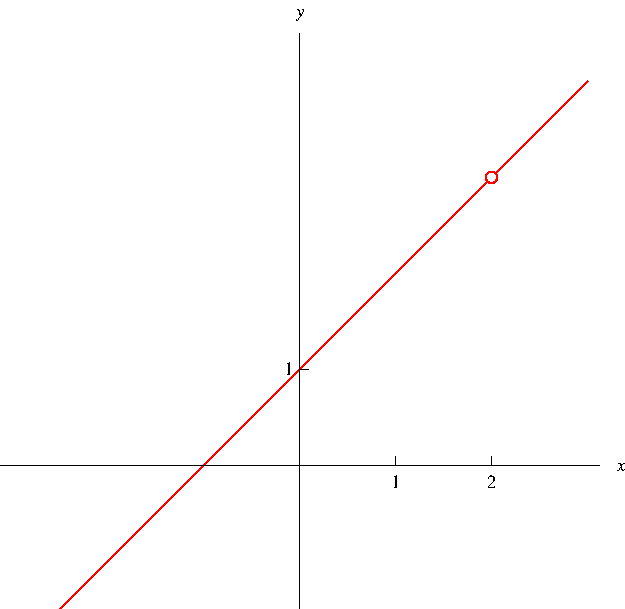
\includegraphics[height=4.5cm]{continuity/pictures/02-05-ex2a.pdf}%
}
\column{.6\textwidth}
\begin{itemize}
\item<2-| alert@2-3>  $f(2)$ \uncover<3->{doesn't exist.}
\item<4->  Discontinuous at 2.
\item<5->  This is called a removable discontinuity because we could remove it by redefining $f$ at the single number 2.
\end{itemize}
\end{columns}
\end{example}
\end{frame}



\begin{frame}
\begin{example}[Example 2b, p. 114]
Where is this function discontinuous?
\begin{columns}[c]
\column{.4\textwidth}
\[
f(x) = \left\{ \begin{array}{lcl}
\frac{1}{\alert<handout:0 |6>{x^2}} & \text{ if } & x \neq 0 \\
\alert<handout:0 |4>{1} & \alert<handout:0 |4>{\text{ if }} & \alert<handout:0 |4>{x = 0} \\
\end{array}\right.
\]
\ 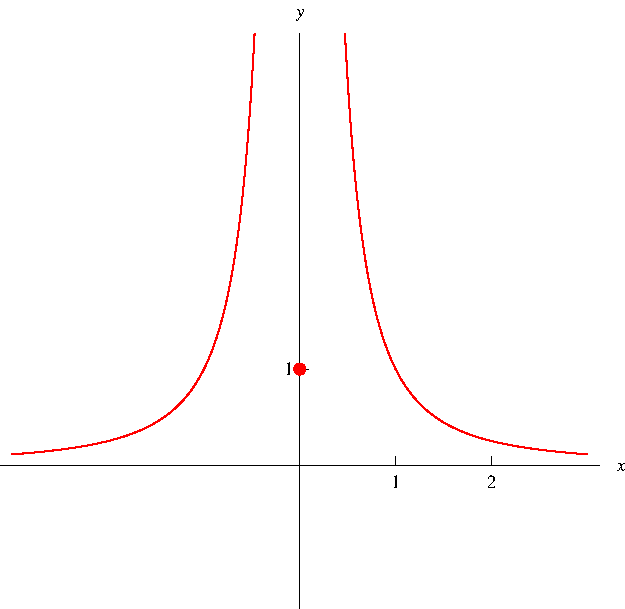
\includegraphics[height=4.5cm]{continuity/pictures/02-05-ex2b.pdf}%
\column{.6\textwidth}
\begin{itemize}
\item<2-| alert@3-4>  $f(0)$ \uncover<4->{exists ($f(0) = 1$).}
\item<2-| alert@5-6>  $\lim_{x\rightarrow 0} f(x)$ \uncover<6->{doesn't exist ($\infty$).}
\item<7->  Discontinuous at 0.
\item<8->  This is called an infinite discontinuity. 
\end{itemize}
\end{columns}
\end{example}
\end{frame}


\begin{frame}
\begin{example}[Example 2c, p. 114]
Where is this function discontinuous?
\begin{columns}[c]
\column{.4\textwidth}
\[
f(x) = \left\{ \begin{array}{lcl}
\frac{x^2 - x - 2}{x-2} & \text{ if } & x \neq 2 \\
\alert<handout:0 |4>{1} & \alert<handout:0 |4>{\text{ if }} & \alert<handout:0 |4>{x = 2} \\
\end{array}\right.
\]
\ 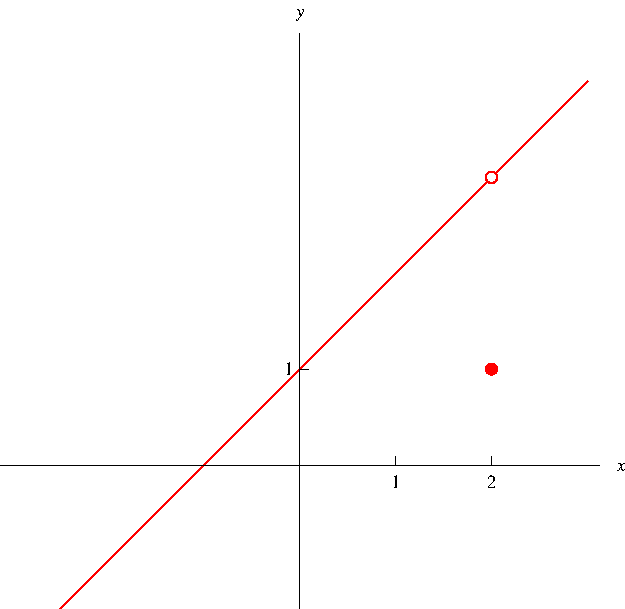
\includegraphics[height=4.5cm]{continuity/pictures/02-05-ex2c.pdf}%
\column{.6\textwidth}
\begin{itemize}
\item<2-| alert@3-4>  $f(2)$ \uncover<4->{exists ($f(2) = 1$).}
\item<2-| alert@5-6>  $\lim_{x\rightarrow 2} f(x)$ \uncover<6->{exists ($3$).}
\item<7->  $\lim_{x\rightarrow 2}f(x) \neq f(2)$.
\item<8->  Discontinuous at 2.
\item<9->  This is also a removable discontinuity.
\end{itemize}
\end{columns}
\end{example}
\end{frame}



\begin{frame}
\begin{example}[Example 2d, p. 114]
Where is this function discontinuous?
\begin{columns}[c]
\column{.4\textwidth}
\[
f(x) = [[x]]
\]
\ 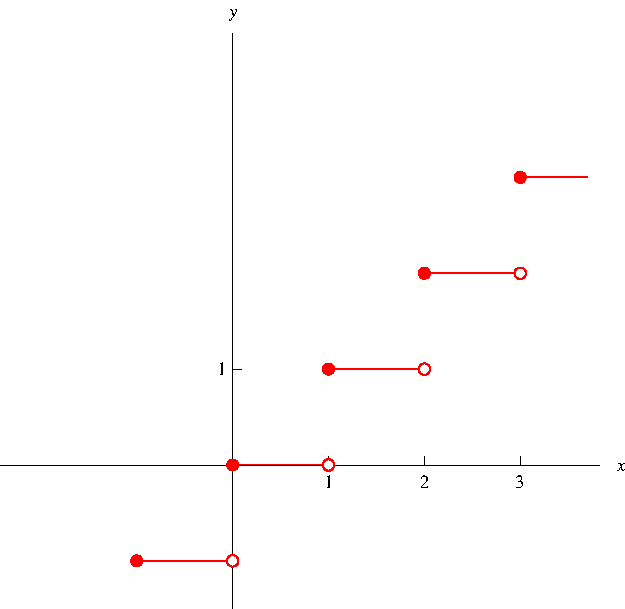
\includegraphics[height=4.5cm]{continuity/pictures/02-05-ex2d.pdf}%
\column{.6\textwidth}
\begin{itemize}
\item<2-| alert@3-4>  $f(1)$ \uncover<4->{exists ($f(1) = 1$).}
\item<2-| alert@5-6>  $\lim_{x\rightarrow 1^+} f(x)$ \uncover<6->{$ = 1$.}
\item<2-| alert@7-8>  $\lim_{x\rightarrow 1^-} f(x)$ \uncover<8->{$ = 0$.}
\item<2-| alert@9-10>  $\lim_{x\rightarrow 1} f(x)$ \uncover<10->{doesn't exist.}
\item<11->  Discontinuous at 1.
\item<12->  Discontinuous at every integer $n$.
\item<13->  These are called jump discontinuities because the function ``jumps'' at these numbers (i.e., the left limit doesn't equal the right limit).
\end{itemize}
\end{columns}
\end{example}
\end{frame}
% end module continuity-ex2

% end lecture

\end{document}
